

\section{Experiments}
\begin{figure*}[ht]
    \centering
    \vspace{-3mm}
    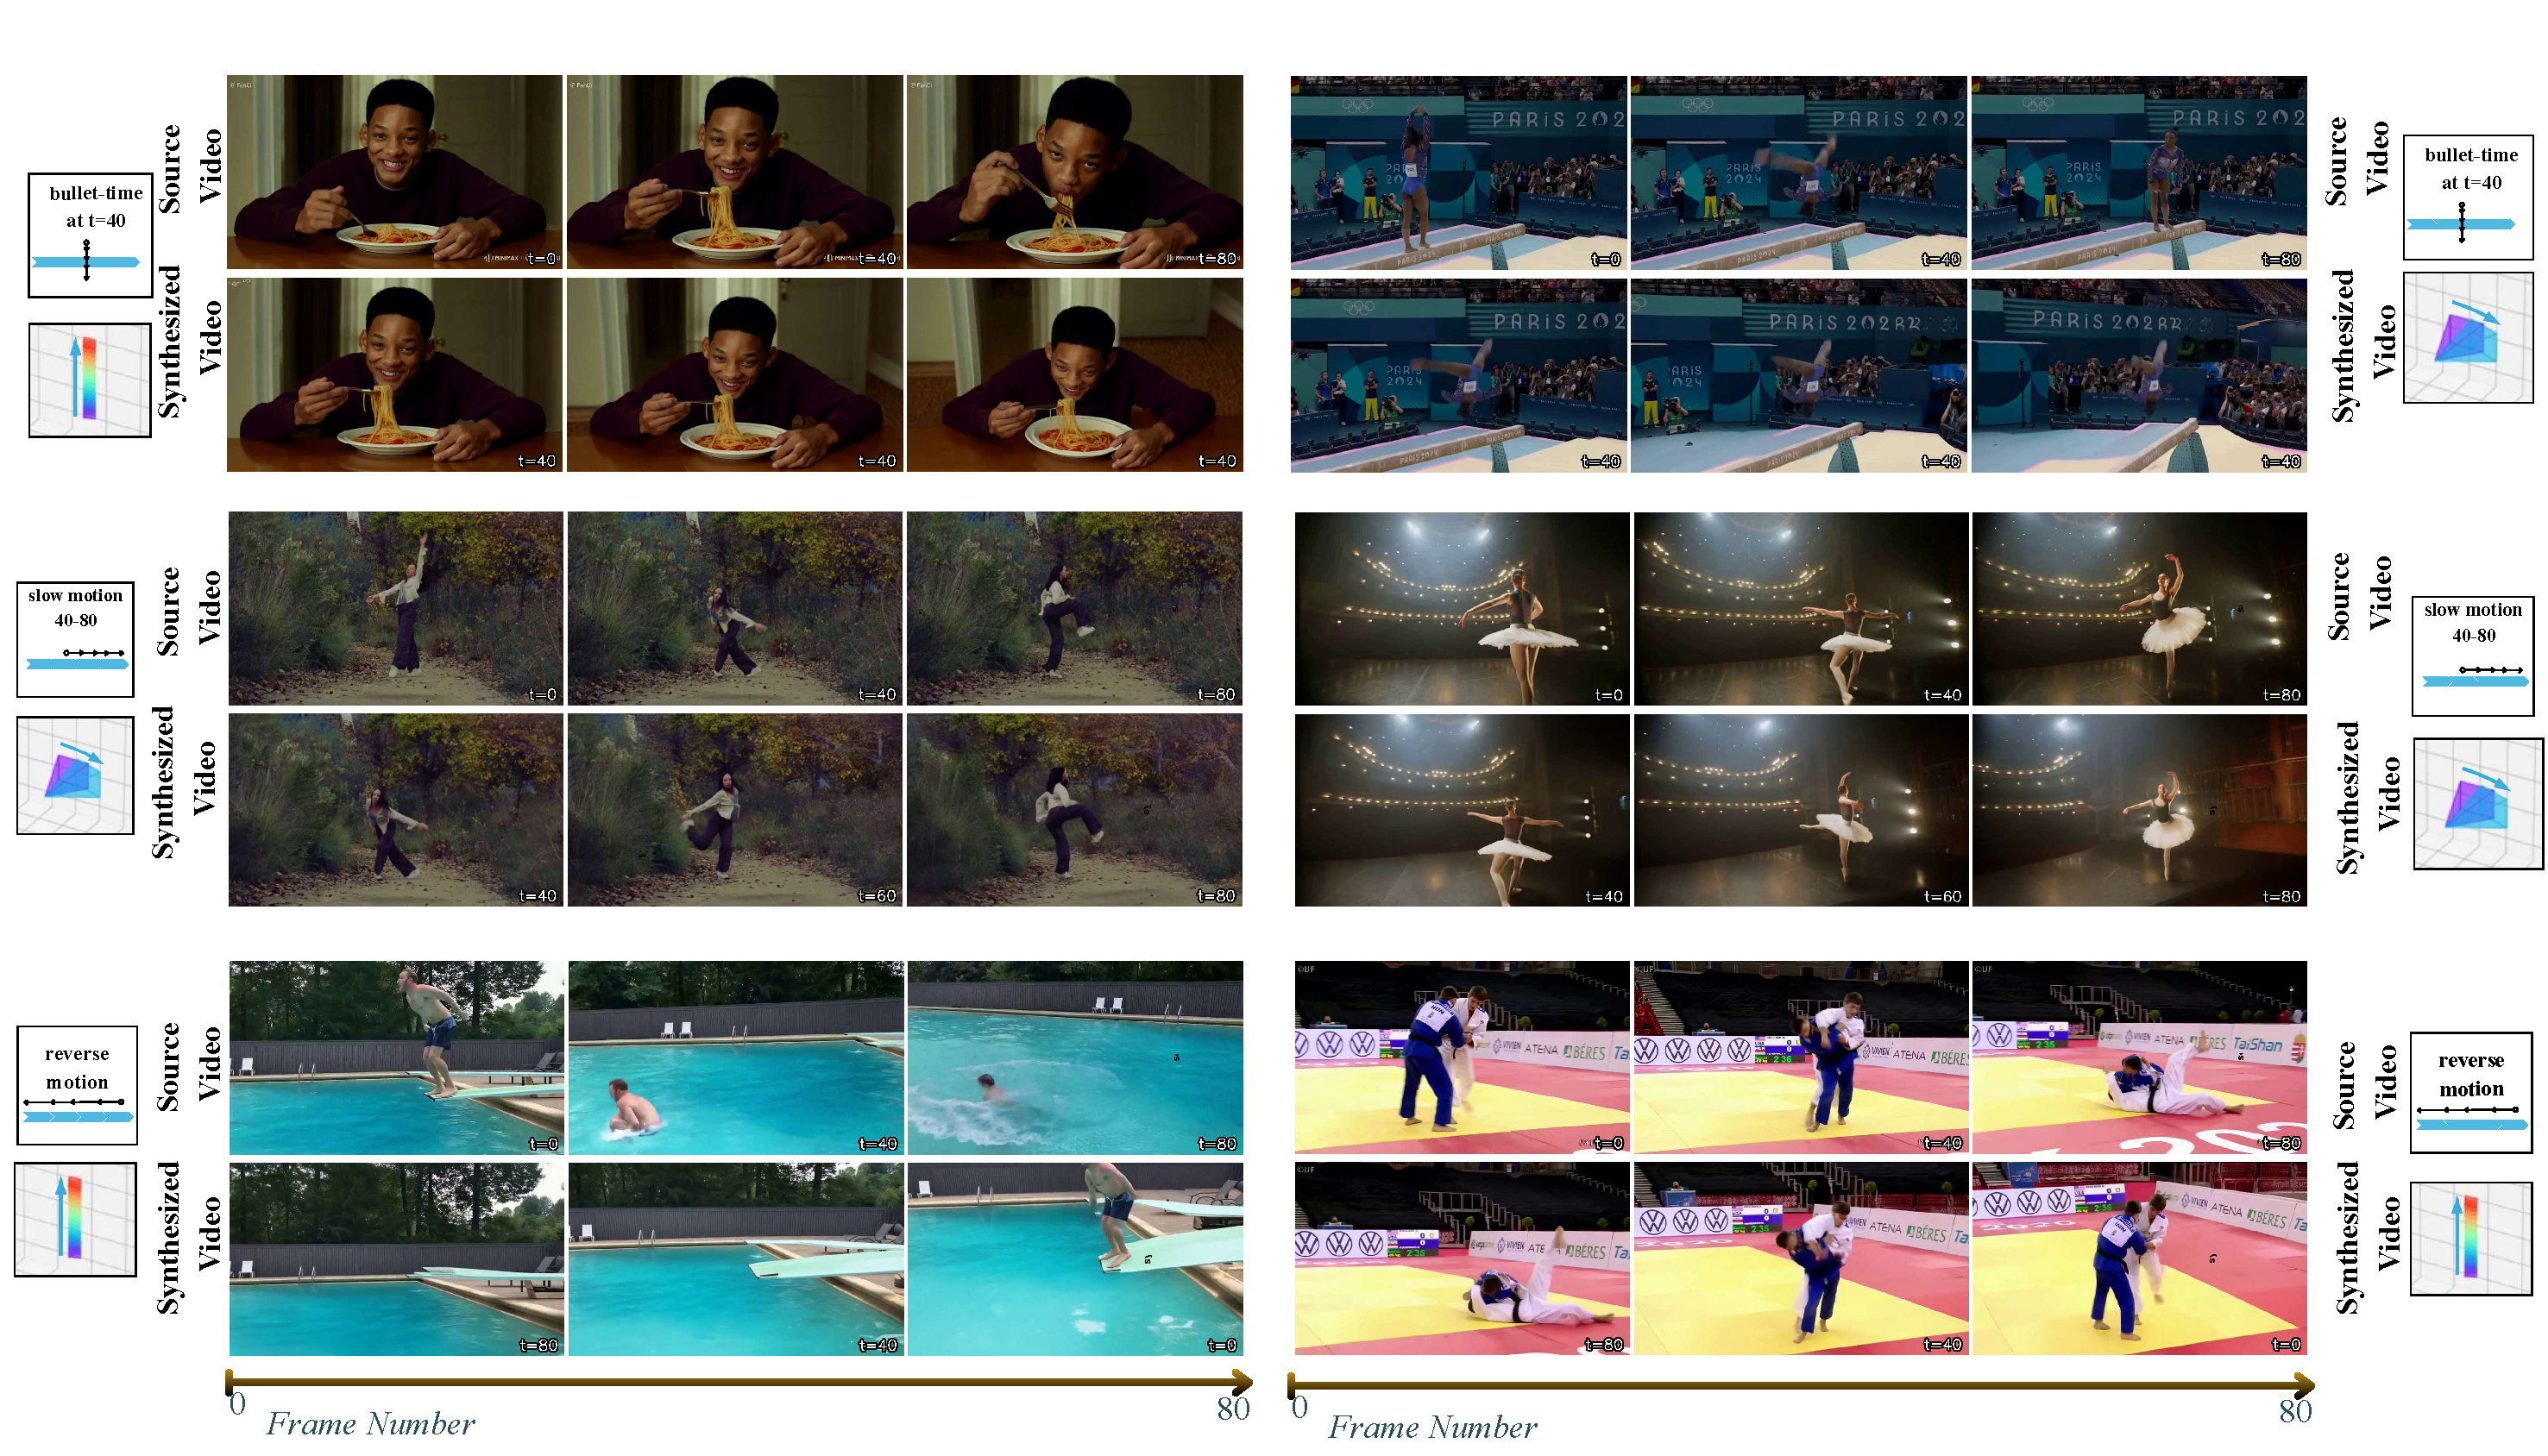
\includegraphics[width=\linewidth]{figures/src_files/example_more.pdf}
    \caption{
    \textbf{Qualitative results of SpaceTimePilot.}
Our model enables fully disentangled control over camera motion and temporal dynamics.
Each row shows a different combination of camera trajectory (left icons) and temporal warping (right icons). SpaceTimePilot produces coherent videos under diverse controls, including normal playback, reverse playback, bullet-time, slow-motion, replay motion, and complex camera paths (pan, tilt, zoom, and vertical motion).
    }
    \label{fig:quali}
\end{figure*}

\myparagraph{Implementation details.}
We adopt the Wan-2.1 T2V-1.3B model \cite{wan2025}, which produces $\numflt$=21 latent frames and decodes them into $\numf$=81 RGB frames using a 3D-VAE.
The network is conditioned on camera and animation-time controls as defined in Eq.~\ref{eq-srccam}.  
Unless otherwise specified, \nameMethod is trained with \recammaster and \syncammaster datasets with the temporal warping augmentation described in Sec.~\ref{sec:datasets}, along with \nameDataset. Please refer to \suppmat for complete network architecture and additional training details.  
\subsection{Comparison with State-of-the-Art Baselines}
\subsubsection{Time-Control Evaluation.}
\label{sec:eval:time_control}
We first evaluate the retiming capability of our model. 
To factor out the error induced by camera control, we condition \nameMethod on a fixed camera pose while varying only the temporal control signal. Experiments are performed on the withheld \nameDataset test split, which contains 50 scenes rendered with dense full-grid trajectories that can be retimed into arbitrary temporal sequences.
For each test case, we take a moving-camera source video but set the target camera trajectory to the first-frame pose. 
We then apply a range of temporal control signals, including reverse, bullet-time, zigzag, slow motion, and normal playback, to synthesize the corresponding retimed outputs. 
Since we have ground-truth frames for all temporal configurations, we report perceptual losses: PSNR, SSIM, and LPIPS.

We consider two baselines:
(1) \textit{ReCamM+preshuffled}: original \recammaster combined with input re-shuffling; and
(2) \textit{ReCamM+jointdata}: following \cite{watson2025controllingspacetimediffusion,Wu2024}, we train \recammaster with additional static-scene datasets \cite{zhou2018stereo,li2019mannequin} which provide only one single temporal pattern.

While frame shuffling may succeed in simple scenarios, it fails to disentangle camera and temporal control.
As shown in Table \ref{tab:temporal_eval}, this approach exhibits the weakest temporal controllability.
Although incorporating static-scene datasets improves performance, particularly in the bullet-time category, relying on a single temporal control pattern remains insufficient for achieving robust temporal consistency.
In contrast, \nameMethod consistently outperforms all baselines across all temporal configurations.

\subsubsection{Visual Quality Evaluation.}
Next, we evaluate the perceptual realism of our 1800 generated videos using VBench \cite{huang2023vbench}. We report all standard visual quality metrics to provide a comprehensive assessment of generative fidelity. 
\Cref{tab:vbench_visual_only} shows that our model achieves visual quality comparable to the baselines.

\begin{table}[t]
    \centering
    \caption{
        VBench visual-quality evaluation across six dimensions.
        Higher is better for all metrics. 
    }
    \vspace{-0.2cm}
    \label{tab:vbench_visual_only}
    \resizebox{\columnwidth}{!}{
    \setlength\tabcolsep{2pt}
    \begin{tabular}{lcccccc}
        \toprule
        \textbf{Method} 
        & ImgQ$\uparrow$ 
        & BGCons$\uparrow$ 
        & Motion$\uparrow$ 
        & SubjCons$\uparrow$ 
        & Flicker$\uparrow$
        & Aesthetic$\uparrow$ \\
        \midrule

        Traj-Crafter \cite{YU2025}
        & 0.6389 & \textbf{0.9376} & 0.9888 & \textbf{0.9463} & 0.9816 & 0.5172 \\

        ReCamM \cite{Bai2025}
        & 0.6302 & 0.9114 & 0.9945 & 0.9181 & \textbf{0.9825} & 0.5332 \\

        ReCamM+Aug
        & 0.6315 & 0.9165 & 0.9946 & 0.9313 & 0.9788 & 0.5385 \\

        \textbf{STPilot (Ours)}
        & \textbf{0.6486} & \textbf{0.9199} & \textbf{0.9947} & \textbf{0.9325} & 0.9781 & \textbf{0.5315} \\
        
        \bottomrule
    \end{tabular}}
\end{table}


\begin{table*}[t]
\centering
\begin{tabular}{cc}

\begin{minipage}{0.55\textwidth}
\centering
\setlength{\tabcolsep}{0.55pt}
{\footnotesize
\caption{Camera accuracy and first-frame estimation. For camera control, the enhanced camera control mechanism enables the generated video to start from an arbitrary camera angle while maintaining good camera accuracy.}
\vspace{-0.2cm}
\label{tab:camera_accuracy}

\begin{tabular}{l|cc|cc||c|cc}
\toprule
\textbf{Method} 
& RelRot$\downarrow$ & RelTrans$\downarrow$ 
& AbsRot$\downarrow$ & AbsTrans$\downarrow$ 
& Rot$^\dagger\downarrow$ 
& RTA15$^\dagger\uparrow$ & RTA30$^\dagger\uparrow$ \\
\midrule
Traj-Crafter \cite{YU2025}  & 5.94 & 0.50 & 6.93 & 0.52 & 9.76 & 22.96\% & 25.93\% \\
ReCamM \cite{Bai2025}      & 4.26 & \textbf{0.32} & 10.08 & 0.34 & 7.49 & 7.61\% & 10.20\% \\
ReCamM+Aug                 & 3.66 & 0.43 & 11.74 & 0.46 & 13.88 & 3.89\% & 5.93\% \\
\textbf{SpaceTimePilot (ours)} 
                           & \textbf{2.71} & 0.33 
                           & \textbf{5.63} & \textbf{0.34} 
                           & \textbf{4.09} 
                           & \textbf{35.19\%} & \textbf{54.44\%} \\
\bottomrule
\end{tabular}
}


\end{minipage}
&
\begin{minipage}{0.43\textwidth}
\centering
\setlength{\tabcolsep}{0.43pt}
{\footnotesize
\caption{Time-embedding compressor ablation. The proposed time-embedding method, trained with temporal warping on the proposed dataset, yields sharper results overall.}
\vspace{-0.2cm}
\label{tab:time_embed_ablation}

\begin{tabular}{lccc}
\toprule
Time Embedding & PSNR$\uparrow$ & SSIM$\uparrow$ & LPIPS$\downarrow$ \\
\midrule
Uniform Sampling     & 14.10 & 0.5981 & 0.5039 \\
1D-Conv              & 14.75 & 0.6134 & 0.4878 \\
1D-Conv + Joint Data & 15.41 & 0.6252 & 0.4830 \\
\textbf{1D-Conv {\small+\nameDataset}} 
                     & \textbf{21.16} & \textbf{0.7674} & \textbf{0.1764} \\
\bottomrule
\end{tabular}
}
\end{minipage}

\end{tabular}

{\footnotesize
\noindent\makebox[\linewidth][l]{$^\dagger$~Evaluation based on first-frame camera accuracy.}
}
\end{table*}













\subsubsection{Camera-Control Evaluation.}
Finlay, we evaluate the effectiveness of our camera control mechanism detailed in Sec.~\ref{sec:src_cam}.
Unlike the retiming evaluation above, which relies on synthetic ground-truth videos, here we construct a real-world 90-video evaluation set from OpenVideoHD~\cite{nan2024openvid}, encompassing diverse dynamic human and object motions.
Each method is evaluated across 20 camera trajectories: 10 starting from the same initial pose as the source video and 10 from different initial poses, resulting in a total of 1800 generated videos.
We apply SpatialTracker-v2~\cite{Xiao2025} to recover camera poses from the generated videos and compare them with the corresponding input camera poses.
\todo{To ensure consistent scale, we align the magnitude of the first two camera locations.}
Trajectory accuracy is quantified using $\mathbf{RotErr}$ and $\mathbf{TransErr}$ following~\cite{He2025camctrl}, under two protocols: (1) evaluating the raw trajectories defined w.r.t.~the first frame (relative protocol, RelRot, RelTrans) and (2) evaluating after aligning to the estimated pose of the first frame (absolute protocol, AbsRot, AbsTrans).
Specifically, we transform the recovered raw trajectories by multiplying the relative pose between the generated and source first frames, estimated by \duster~\cite{dust3r_cvpr24}. 
We also compare this \duster pose with the target trajectory’s initial pose, and report RotErr, RTA@15 and RTA@30, as translation magnitude is scale-ambiguous.

\begin{figure}[t]
    \centering
    \vspace{-3mm}
    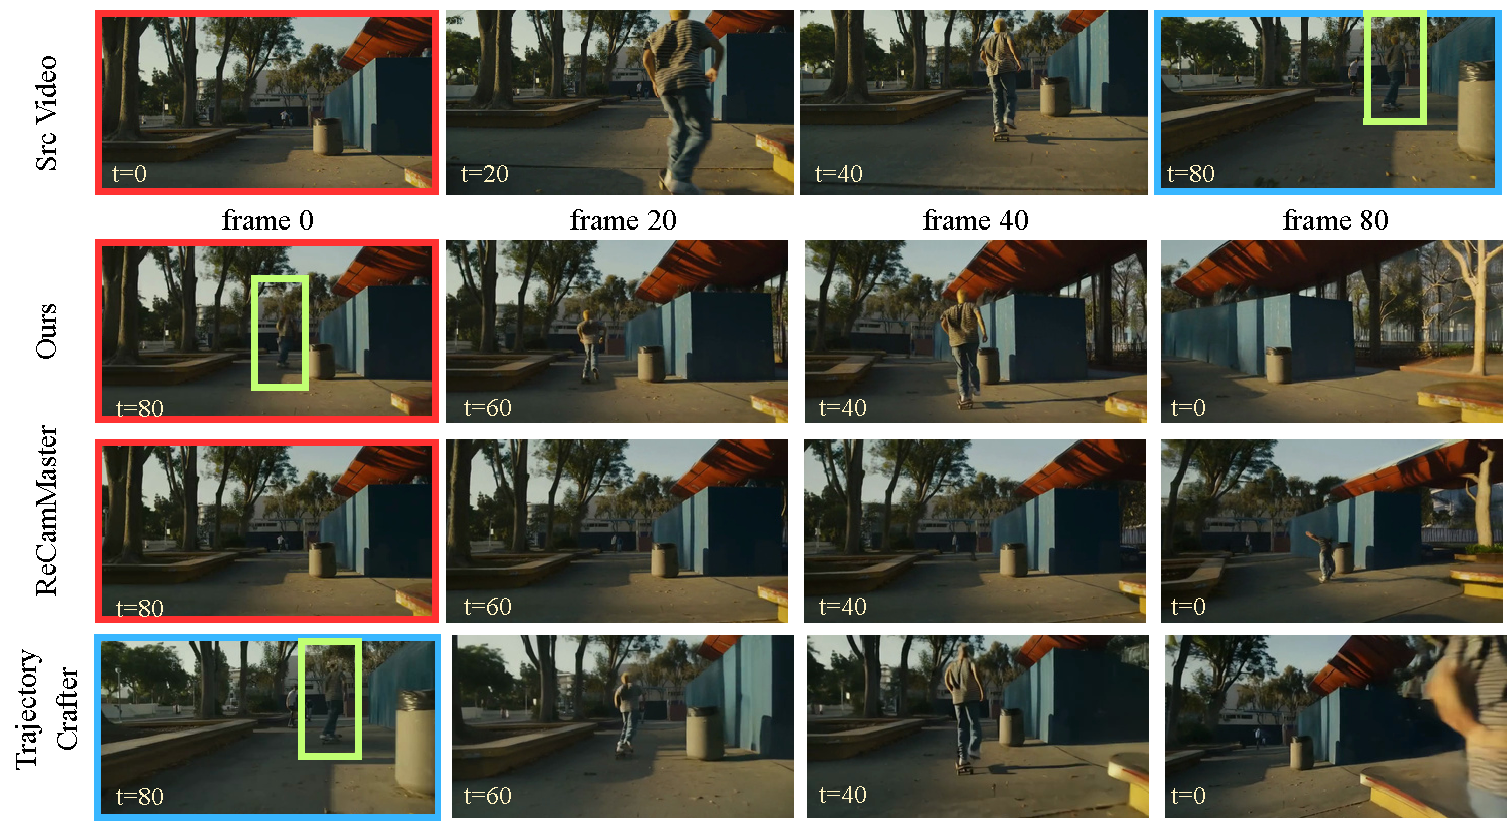
\includegraphics[width=\linewidth,trim={0 0 0 0},clip]{figures/src_files/Comparison_2.pdf}
    \caption{
    \textbf{Qualitative comparison of disentangled camera-time control.}  In this example, we apply reverse playback (time) and a pan-right camera motion starting from the first-frame pose to a source video (top), whose original camera motion is dolly-in (red to blue). SpaceTimePilot, by explicitly disentangling space and time, achieves correct camera control (red boxes) together with accurate temporal control (green boxes). For TrajectoryCrafter, it  first reverses the frames and then apply their method for viewpoint control, resulting in incorrect  camera motion. ReCamMaster (with joint-dataset training) is unable to perform temporal control, leading to failure cases.}
    \label{fig:disentangle}
\end{figure}




\begin{figure}[t]
    \centering
    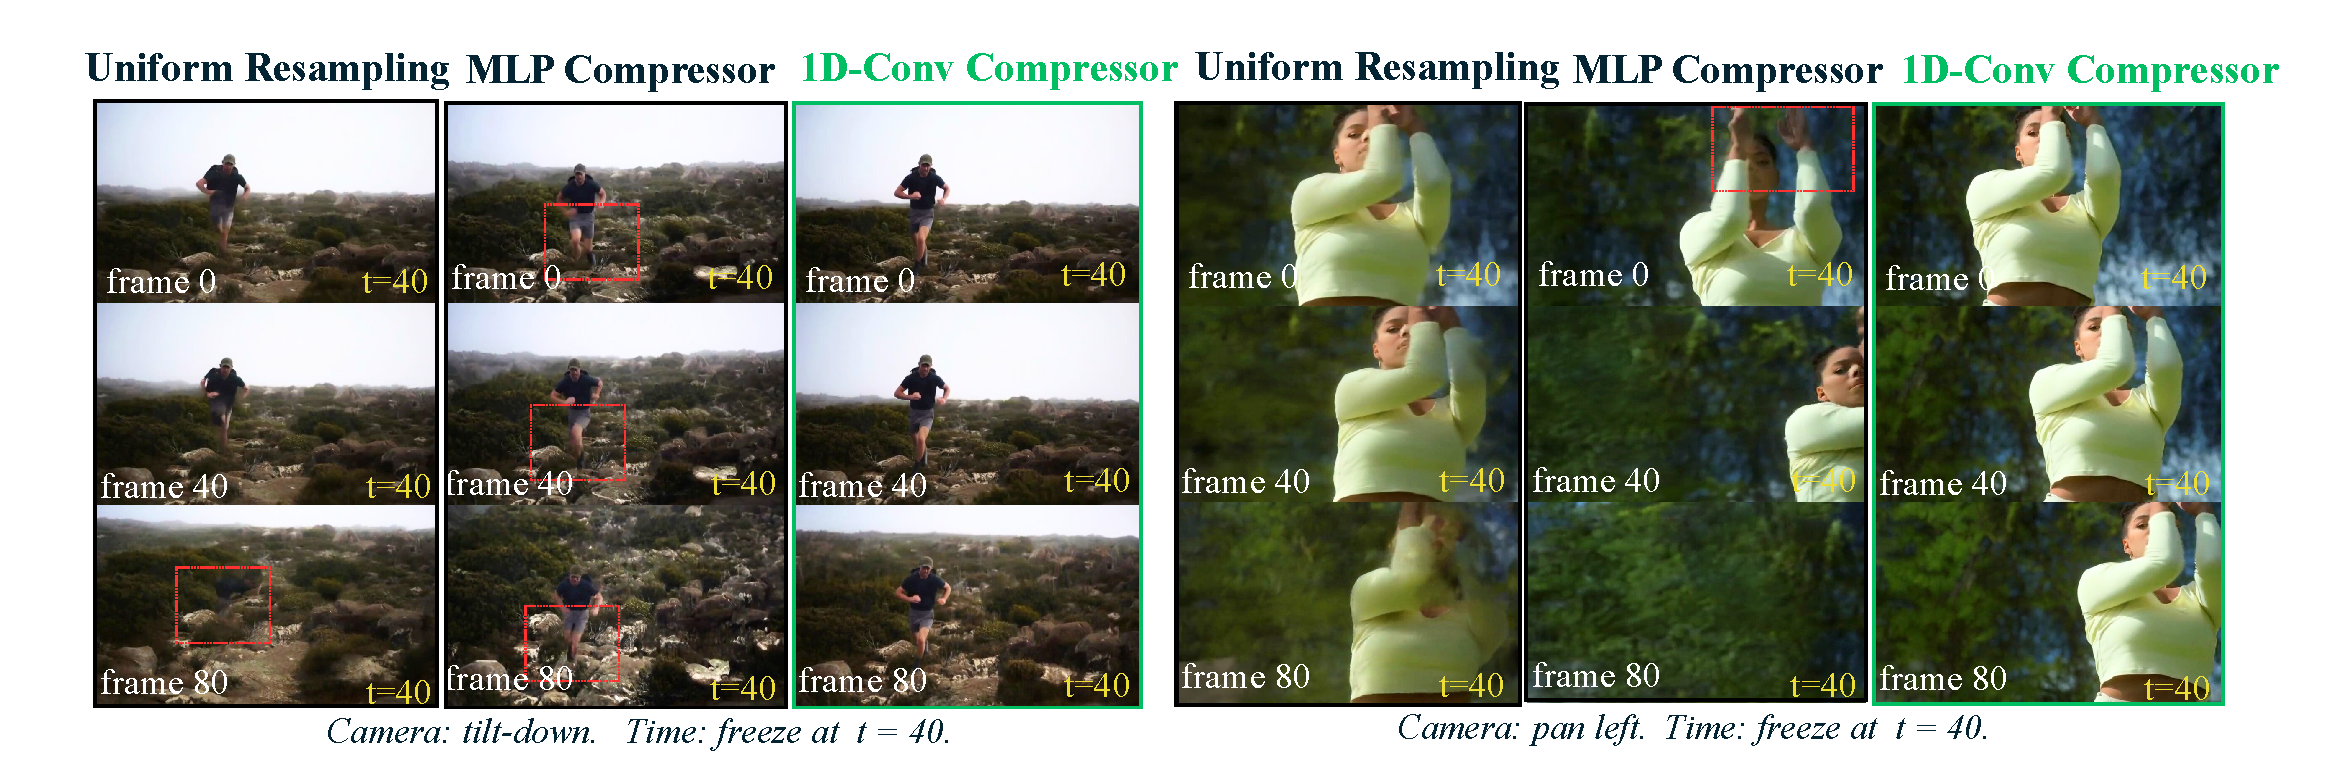
\includegraphics[width=1\linewidth, trim={5mm 5mm 5mm 1mm}, clip]{figures/time_emb_ablation.pdf}
    \caption{
        \textbf{Temporal compression ablation.}
        Comparing uniform resampling, MLP, and 1D-Conv compressors under tilt-down and pan-right bullet-time controls, $\animatime_\trg = [40,\dots,40]$.
    }
    \label{fig:temporal_ablation}
\end{figure}


To measure only the impact of source camera conditioning, we consider the original \recammaster~\cite{Bai2025} (\textit{ReCamM}) and two variants. 
Since \recammaster is originally trained on datasets where the first frame of the source and target videos are identical, the model always copies the first frame regardless of the input camera pose. 
For fairness, we retrain \recammaster with more data augmentations to include non-identical first frames, denoted as \textit{ReCamM+Aug}. 
Next, we condition the model additionally with source cameras $\camera_\src$ following Eq.~\ref{eq-srccam}, denoted as \textit{ReCamM+Aug+$\camera_\src$}. 
Finally we also report the results of TrajectoryCrafter~\cite{YU2025}.

In Table~\ref{tab:camera_accuracy}, we observe that the absolute protocol produces consistently higher errors, as trajectories must not only match the overall shape (relative protocol) but also align correctly in position and orientation.
Interestingly, ReCamM+Aug yields higher errors than the original ReCamM, whereas incorporating source cameras $\camera_\src$ results in the best overall performance.
This suggests that, without explicit reference to $\camera_\src$, exposure to more augmented videos with differing initial frames can instead confuse the model.
The newly introduced conditioning signal on the source video’s trajectory $\camera_\src$ achieves substantially better camera-control accuracy across all metrics, more reliable first-frame alignment, and more faithful adherence to the full trajectory than all baselines. 

\subsubsection{Qualitative results.}
Besides the quantitative evaluation, we also demonstrate the strength of \nameMethod with visual examples.
In \cref{fig:disentangle}, we show that only our method correctly synthesizes both the camera motion (red boxes) and the animation-time state (green boxes). While \recammaster handles camera control well, it cannot modify the temporal state, such as enabling reverse playback. TrajectoryCrafter, in contrast, is confused by the reverse frame shuffle, causing the camera pose of the last source frame (blue boxes) to incorrectly appear in the first frame of the generated video. More visual results can be found in \cref{fig:quali}.
\subsection{Ablation Study}

\label{sec:time_embedding_ablation}
To validate the effectiveness of the proposed Time embedding module, in Table \ref{tab:time_embed_ablation}, we follow the time-control evaluation set up in Sec.~\ref{sec:eval:time_control} and compare our 1D convolutional time embedding against several variants and alternatives discussed in Sec.~\ref{sec:time_embedding}:
(1) Uniform-Sampling: sampling the 81-frame embedding uniformly to a 21-frame sequence, which is equivalent to adopting sinusoidal embeddings at the latent frame $f'$ level;
(2) 1D-Conv: using 1D convolution layers to compress from $\animatime \in \mathbb{R}^F$ to $\animatime \in \mathbb{R}^{F'}$, trained with ReCamMaster and SynCamMaster datasets.
(3) 1D-Conv+jointdata: row 2 but including additionally static-scene datasets \cite{zhou2018stereo,li2019mannequin}.
(4) 1D-Conv (ours): row 2 but instead including the proposed \nameDataset.  
We observe that applying a 1D convolution to learn a compact representation by compressing the fine-grained $\numf$-dim embeddings into a $\numflt$-dim space performs notably better than directly constructing sinusoidal embeddings at the coarse $f'$ level.
Incorporating static-scene datasets yields only limited improvements, likely due to their restricted temporal control patterns.
By contrast, using the proposed \nameDataset consistently delivers the largest gains across all three metrics, confirming the effectiveness of our newly introduced datasets.
Furthermore, as shown in \cref{fig:temporal_ablation}, we present a visual comparison of bullet-time results using uniform sampling and an MLP instead of the 1D convolution for compressing the temporal control signal.
Uniform sampling produces noticeable artifacts, and the MLP compressor causes abrupt camera motion, whereas the 1D convolution effectively locks the animation time and enables smooth camera movement.












